% Source schematic: 2006 Fujian arts paper, Q20, source PDF page 2.
% Include inside a document that loads TikZ.
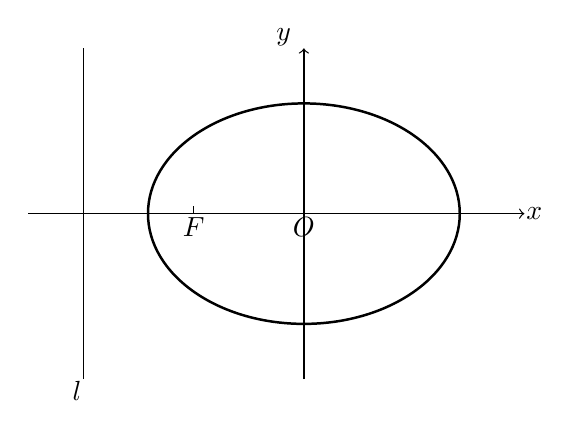
\begin{tikzpicture}[x=1.4cm,y=1.4cm,line cap=butt,line join=round]
  % Coordinate axes: arrows point in the positive directions only.
  \draw[->,line width=0.45pt] (-2.5,0) -- (2,0);
  \draw[->,line width=0.45pt] (0,-1.5) -- (0,1.5);

  % Left directrix, shown as a plain solid vertical line.
  \draw[line width=0.45pt] (-2,-1.5) -- (-2,1.5);

  % Ellipse x^2/2 + y^2 = 1, with the left focus tick on the x-axis.
  \draw[line width=0.9pt] (0,0) ellipse [x radius=1.4142,y radius=1];
  \draw[line width=0.45pt] (-1,0) -- (-1,0.07);

  % Labels copied from the schematic.
  \node[above left,inner sep=0.5pt] at (-0.1,1.5) {$y$};
  \node[right,inner sep=0.5pt] at (2,0) {$x$};
  \node[below,inner sep=0.5pt] at (-1,-0.02) {$F$};
  \node[below,inner sep=0.5pt] at (0,-0.02) {$O$};
  \node[below left,inner sep=0.5pt] at (-2,-1.5) {$l$};
\end{tikzpicture}
